\section{Evaluation Study}

The flow of the study for our participants in the EP is shown in Fig.~\ref{fig:studyflow}. 
The elements inside the curly braces occurred within the mobile app. 
In the app, in addition to linking to the online surveys, users completed the five-round ``gameplay'' titled Monster Munch. The DCP served as a method of data collection for use in the EP, as well as an opportunity for the research team to evaluate possible changes and improvements to the study plan and opportunities for data analysis. The difference between the DCP and EP can be seen in Fig.~\ref{fig:phasechart}.

\subsection{Participants}

For the DCP, participants were recruited from Amazon Mechanical Turk (AMT) with the following inclusion criteria: 1) Own an Android mobile device, 2) Are above 18 years of age (self-reported on AMT).

After accepting the terms of the study found in the consent form, participants were asked to download an APK file where they completed the pre-task, the nutritional task of the simplified app, and the post-task. 

For the EP, recruitment was conducted through both AMT and social media sites (e.g., Twitter, Instagram, Facebook, and LinkedIn).
% Include here or in Results?%
% The participants were divided into two groups based on their highest level of educational achievement. Participants with a highest level of educational attainment of high school/GED and below make up the Low Education Users (LEU), n=??. The High Education Users (HEU) are comprised of participants with a highest level of educational attainment of some college and higher.
The inclusion criteria from the DCP was used for both groups : 1) Own an Android mobile device, 2) Are above 18. 


Among the total recruited population,
(\textit{$N_{control}$} = 54, \textit{$N_{treatment}$} = 68; \textit{$N_{total}$} = 122). The study was approved by two east coast universities' Internal Review Boards as they collaborated on this project.

\textcolor{red}{SAMPLE WRITING:} `` participated in our study through Amazon Mechanical Turk (MTurk), a platform that acts as a broker
between parties offering a range of Human Intelligence
Tasks (HITs) (e.g., marketing questionnaires or research
studies) and paid workers. Participants received \$6 compensation paid through the platform. Although it has been
shown that MTurk is a reliable research tool [38], we measured the time spent per questionnaire to evaluate task performance and ensure that participants were attentive despite
the online setting [23]. Participants were excluded from
further analysis based on the following: if participants filled
in more than 2 surveys with zero variance between items, or
showed ratings of ±3SD in more than 2 questionnaires. After these filters were applied, 126 participants (38.9\% female) with an average age of 31.61 (SD=8.20) were included in further analysis. Excluding participants based on quality criteria is a standard approach for data collected via
crowdsourcing platforms; the applied criteria were suggested by [38]. ''


\subsection{Research Questions and Hypotheses}

\begin{enumerate}
    \item Does playing the Meal for Monsters game help users better assess the ``right'' in-the-wild meals to meet specific macronutrient nutritional goals?
    \item Does player-avatar identification in the Meals for Monsters game relate to user learning and experience?
    \item Do users utilize the crowdsourced intelligence or community's feedback when making meal choices?
\end{enumerate}

The hypotheses are:
\begin{itemize}
    \item \textbf{H1}: Meal for Monsters (a pet avatar health game with crowdsourced meal photographs) will help users learn to identify the ``right'' in-the-wild meals for a specific nutritional goal (e.g., reduction of fat, increase in carbohydrates) pre to post-test.
    \item \textbf{H2}: Players who choose pet avatars with a health goal that is personally meaningful in Meals for Monsters are more likely to perform better (i.e., identify the right meal photographs for a specific nutritional goal) pre to post test and show enthusiasm towards the game. 
    \item \textbf{H3}: Over time players will consider the community or crowdsourced wisdom on choosing the ``right'' meals for a specific macronutrient nutritional goal.

\end{itemize}

\subsection{Study Design}

\begin{figure}[h]
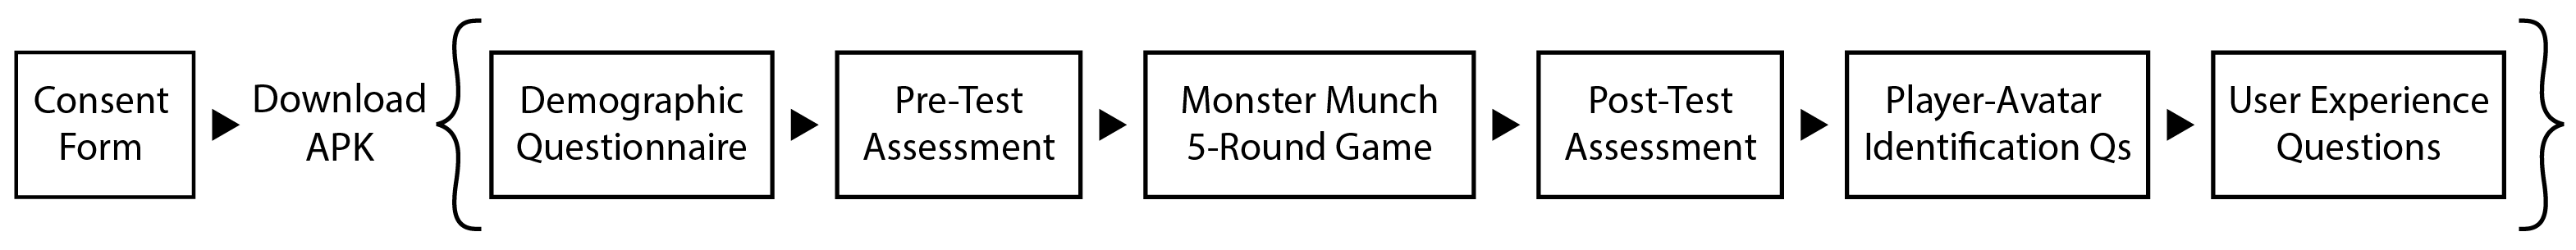
\includegraphics[width=\textwidth]{samples/images/figure-1.png}
\caption{Graphic showing the flow of the study for the Treatment Group.}
\label{fig:studyflow}
\end{figure}

\subsubsection{Data Collection Phase (DCP)}

The three primary goals of the DCP were to 1) collect user-generated responses to use within the `Monster Munch' community board in the EP, 2) provide initial insights on the prior knowledge and nutritional literacy of lay users, and 3) assess the user experience and data collection methods of the game. 
To accomplish these goals, users in the DCP completed both a pre-task and post-task, and a simplified version of the more complete app used in the EP.


\subsection{Data Collection}

In Phase 1, every user will be assigned one of the four pet monsters, each having their own nutritional goal. 
The user will be introduced to their monster avatar and nutritional goal before proceeding to the five rounds. 
There will be three steps for the user in each of the five rounds. 
First, the user will be presented with the four options of ``in-the-wild'' meal photographs, accompanied with brief descriptions of the contents of each meal, where they will select the meal that they believe best fits their pet monster’s nutritional goal. 
Next, the user will be asked to provide a short description of why they selected that particular option. 
Finally, after the user submits their reasoning, the game will show them whether the meal option they selected was correct, and if they were incorrect, which meal option was the best choice. 
Each user will repeat these three steps for all five rounds with the same pet monster and its nutritional goal. 

\subsection{Phase 2}

The game in Phase 2 differs from the previous phase with the addition of three key features.


\subsubsection{Preparation}

To prepare for Phase 2, the three key features will be programmed into the M4M game.
We will also filter the user-generated responses from Phase 1 for relevancy and grammatical accuracy. 
The filtered responses will then be used to create the community board for users to view in the game. 
The community board will also feature the calculated percentages of Phase 1 users that selected each meal choice per round.
Along with the creation of the community board, we will amend additional questions to the post-task survey that relate to the added features of the game. 
Since users will be able to select their own monster avatar in this phase, we will ask questions regarding the reason why they chose their avatar. 
We will also ask participants a series of relevant questions from the Player-Avatar Identification Scales~\cite{li2013player} using a 5-point Likert scale. 

\subsubsection{Data Collection}


In Phase 2, users now have the ability to view each of the four pet monster avatars and their nutritional goals before selecting one to proceed with and care for during the game. The user will also have the opportunity to give their monster a custom name. 
Then, there will be five steps for the user in each of the five rounds. 
First, after the user is presented with the four options of in-the-wild meal photographs, accompanied with brief descriptions of the contents of each meal, they will select the meal that they believe best fits their monster’s nutritional goal.  
Second, the user will then be asked to provide a short description of why they selected that particular option. 
Third, the user will be shown the community board of crowdsourced reasons why other users selected one of the four meal options. With this new information, the user will have the option to keep their original meal selection, or switch to one of the other meals.
Fourth, the user will be asked to provide a short description of why they selected that meal option.
Last, after they submit their reasoning, the game will show the user whether the meal option they selected was correct, and if they were incorrect, which meal option was the best choice. 
As described earlier in Key Feature 3, depending on the how successful the user has been, the results also include either a short animated morph of the pet monster reacting to the meal the user fed them or the ability for the user to choose an accessory for their pet monster.
Each user will repeat these five steps for all five rounds with the same pet monster and nutritional goal.
%%% Is this sort of thing needed for CHI?%%%
%\subsection{Analysis}
%We will use a combination of qualitative and quantitative methods to analyze the data collected during the proposed study. For the quantitative measures collected during the study (results of their scores on different questionnaires and accuracy of their nutritional assessment), we will use appropriate statistical tests to examine the differences in means for the measures of interest.


